\documentclass[conference]{IEEEtran}

\usepackage{amsmath,amssymb}
\usepackage{booktabs}
\usepackage{graphicx}
\usepackage[caption=false,font=footnotesize]{subfig}
\usepackage{microtype}
\usepackage{url}
\usepackage{xcolor}

\newcommand{\E}{\mathbb{E}}
\newcommand{\norm}[1]{\left\lVert#1\right\rVert}
\newcommand{\ind}[1]{\mathbf{1}_{\{#1\}}}
\newcommand{\vect}[1]{\boldsymbol{#1}}
% Set \showrevisionsfalse for the anonymous submission PDF.
\newif\ifshowrevisions
\showrevisionstrue
\definecolor{spacegreen}{RGB}{0,110,75}
\definecolor{actionorange}{RGB}{180,80,0}
\ifshowrevisions
  \newcommand{\rev}[1]{{\color{blue}#1}}
  \newcommand{\prov}[1]{{\color{red}#1}}
  \newcommand{\newrev}[1]{{\color{violet}#1}}
  \newcommand{\spacerev}[1]{{\color{spacegreen}#1}}
  \newcommand{\actionrev}[1]{{\color{actionorange}#1}}
\else
  \newcommand{\rev}[1]{#1}
  \newcommand{\prov}[1]{#1}
  \newcommand{\newrev}[1]{#1}
  \newcommand{\spacerev}[1]{#1}
  \newcommand{\actionrev}[1]{#1}
\fi
\newtheorem{proposition}{Proposition}
\newtheorem{theorem}{Theorem}
\newtheorem{algorithm}{Algorithm}

\title{Event-FedAvg: Stateful Event-Driven Communication for Federated Learning}

% Keep the initial submission anonymous if required by the final IJCNN 2027
% author instructions. Author identities and affiliations are added only after
% the applicable submission policy is verified.
\author{\IEEEauthorblockN{Anonymous Authors}}

\begin{document}
\maketitle

\begin{abstract}
\spacerev{Federated learning repeatedly exchanges high-dimensional updates even
when individual model parameters change only slightly per round. Event-FedAvg
instead accumulates weighted local-model changes in leaky client states and
emits signed events only when a parameter state crosses a threshold. The server
sums simultaneous events parameterwise and applies an independently scheduled
model quantum, allowing opposing events to cancel. A sparse replay or, when
cheaper, a complete checkpoint then synchronizes all clients. We prove a
pathwise state and event-budget bound and a conditional finite-horizon bridge
from event alignment to gradient norm. A pulse-level decomposition and alignment study connect
heterogeneity and local-update depth to finite-trajectory behavior. Under
matched local training, development-only tuning, and bidirectional traffic
accounting, Event-FedAvg is nondominated in the observed mean
communication--accuracy plane across Fashion-MNIST MLP/CNN and CIFAR-10
CNN/ResNet-14 experiments. A matched-traffic operator audit identifies
cross-round persistence, rather than the precise reset rule, as the influential
encoder choice at the audited operating point. Across ten paired ResNet-14 seeds, it
reaches $75.14\pm0.90\%$ accuracy at $38.66\pm0.36$ Gbit, compared with
$74.21\pm0.74\%$ at $336.56$ Gbit for development-tuned dense FedAvg. These
results establish a communication--performance operating point in the evaluated
synchronous setting, not unconditional convergence or hardware-energy savings.}
\end{abstract}

\section{Introduction}
\label{sec:introduction}

Federated learning (FL) allows a fleet of clients to improve a shared model
without collecting their raw data at one location. Keeping data local,
however, does not make the optimization process communication-free. Every
training round may require high-dimensional client uploads followed by a server
message that brings all clients to the next common model. For bandwidth-limited
edge systems, this repeated exchange can become the main scaling bottleneck of
federated averaging (FedAvg) \cite{mcmahan2017fedavg}.

\spacerev{A model parameter may change too little to justify transmission in a
single round, yet consistently directed changes can accumulate over time.
Round-wise compression does not directly exploit this persistence.
Error-feedback instead stores discarded compression residuals for later
correction~\cite{stich2018memory,richtarik2021ef21}. This motivates our design
question: \emph{Can each client integrate weak parameter-wise updates and
communicate only when their accumulated state crosses a threshold?}}

\spacerev{Event-FedAvg is a stateful communication layer for a conventional
model and optimizer. Inspired by leaky integrate-and-fire neurons
\cite{gerstner2014neuronal}, its client encoder retains part of a parameter-wise
state, adds new local evidence, emits an index and sign at a threshold, and
resets. An independent \emph{model quantum} determines how far each net event
moves the server parameter.}

\spacerev{After every round, the server synchronizes all clients by returning
either the ordered sparse update sequence or, when cheaper, a complete model
checkpoint. Thus every client begins the next round from the same model, even
when no event was emitted.}

\spacerev{We contribute the complete encoder, server update, and synchronization
algorithm rather than claiming its individual ingredients as new. We establish
pathwise state and event-budget guarantees, derive a conditional bridge from
event alignment to finite-horizon gradient norm, and decompose alignment into
measurable mechanisms. A matched-traffic operator audit shows that removing
cross-round memory reduces accuracy by $11.64$ points on the compact CIFAR-10
CNN, while subtractive reset changes it by only $+0.42$ points and uses more
traffic. Ten-seed comparisons against four referenced baselines use matched
local training and total bidirectional traffic. Event-FedAvg is nondominated
among the evaluated mean operating points in all four settings. On CIFAR-10 ResNet-14, it
uses $8.7\times$ less traffic than dense FedAvg while improving mean accuracy
by $0.93$ percentage points. Figure~\ref{fig:event-fedavg-method} summarizes a
complete round.}

\section{\rev{Related Work}}
\label{sec:related-work}

\spacerev{One-bit, sign, and sparse methods reduce message precision or density,
while memory and error feedback preserve discarded residuals
\cite{seide2014onebit,bernstein2018signsgd,stich2018memory,richtarik2021ef21}.
Sparse Ternary Compression applies residual-corrected sparsification in both FL
directions~\cite{sattler2020stc}. Strom's parameter-wise residuals and signed
threshold pulses are the closest predecessor~\cite{strom2015distributed}.
Event-FedAvg instead leaks old evidence, fully resets fired states, and separates
the trigger threshold from the server quantum.

\actionrev{Event-triggered learning suppresses a vector until a model or
gradient deviation is sufficiently large
\cite{ghadikolaei2021lena,singh2023sparq,he2023etfl,yoon2025etfl,
zhai2026gossip}. LENA uploads accumulated vector memory, SPARQ-SGD retains
stale neighbor estimates, and ETFL-family methods trigger model or gradient
messages. They do not combine parameter-wise sign events with an independently
scheduled server quantum and exact replay-or-checkpoint synchronization.
Event-FedAvg's contribution is this complete operator and protocol. We do not
claim novelty for accumulation, thresholding, sign transmission, leakage, or
full reset individually. EF-TopK and Sign-EF cover the retained-residual and
sign-quantization mechanisms used by STC, although we do not implement STC's
data-dependent ternary magnitude.}
Federated spiking-neural-network work trains models whose neurons exchange
spikes and maintain LIF states
\cite{venkatesha2021fedsnn,chaki2023tradeoffs,tao2026sfedhifi}. Here, the
LIF-inspired state belongs only to the communication layer around a
conventional model.}

\begin{figure*}[!t]
 \centering
 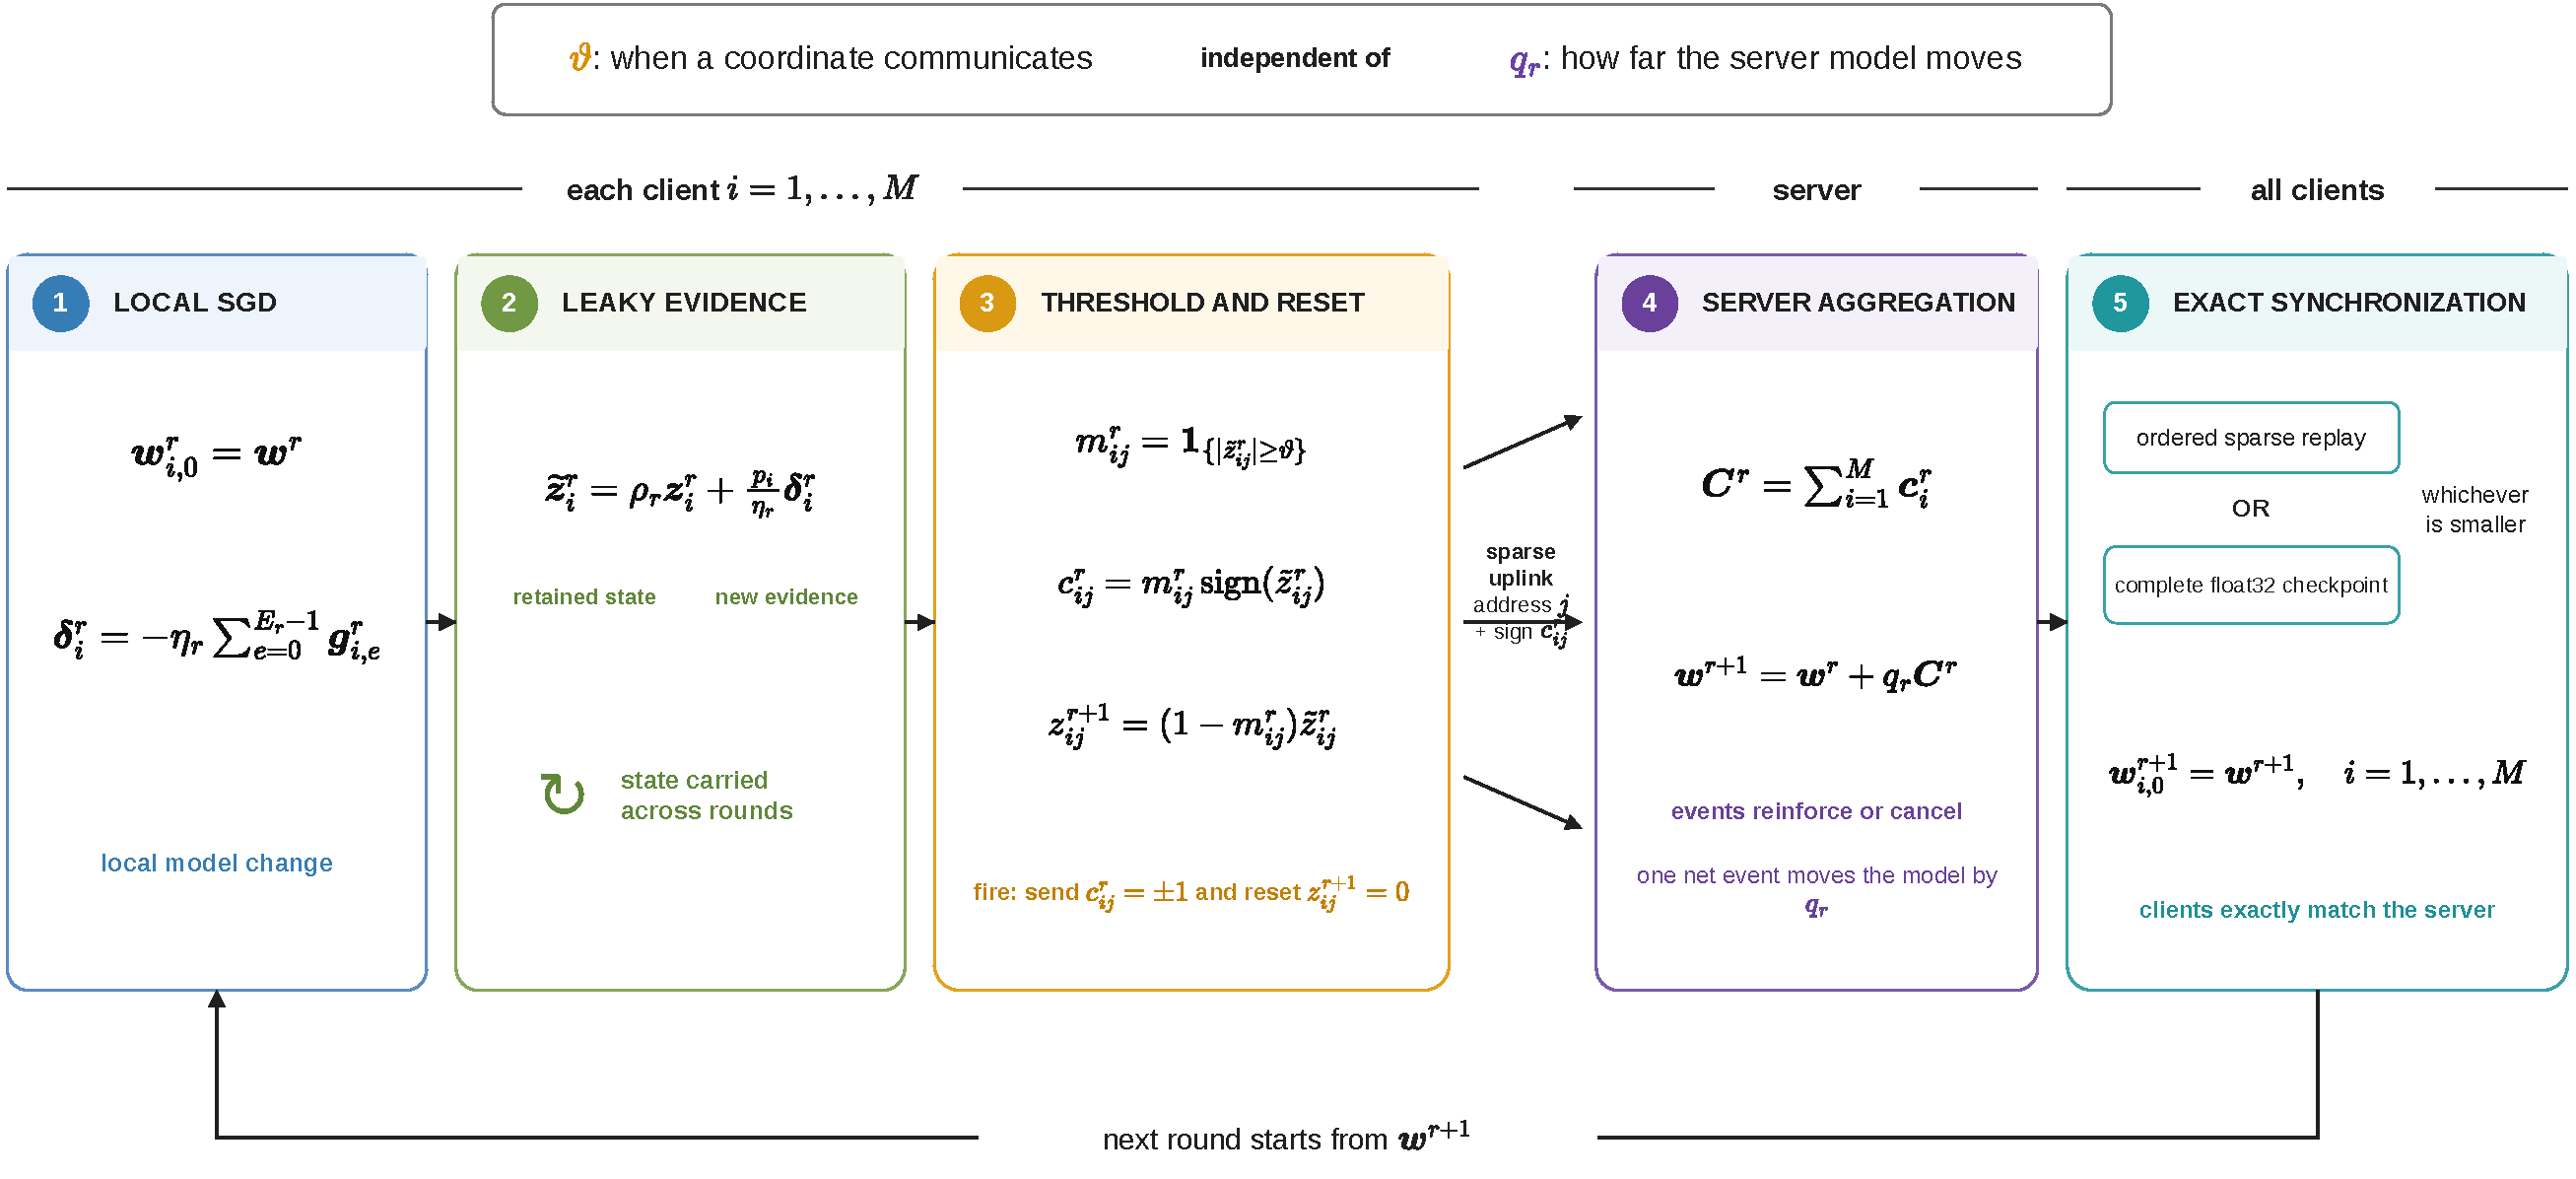
\includegraphics[width=0.88\textwidth]{figures/event_fedavg_method.pdf}
 \caption{\spacerev{Event-FedAvg accumulates weighted local changes in leaky
 client states, emits signed threshold events, and scales their server aggregate
 by the independent quantum $q_r$. After every round, ordered replay or a
 checkpoint synchronizes all clients.}}
 \label{fig:event-fedavg-method}
\end{figure*}

\section{Event-FedAvg}
\label{sec:method}

\spacerev{We follow one round from local training through event encoding to the
server update and downlink synchronization.}

\subsection{Round notation and local update}

Let rounds be indexed by $r\in\{1,\ldots,R\}$, clients by
$i\in\{1,\ldots,M\}$, and model coordinates by $j\in\{1,\ldots,d\}$, where a
coordinate is one scalar model parameter.
The server model at the start of round $r$ is
$\vect{w}^r\in\mathbb{R}^d$, and every client starts from this same model.
Client $i$ has local objective $F_i$ and aggregation weight $p_i>0$, with
$\sum_i p_i=1$. \newrev{The weights are protocol parameters known to the
server and clients before training. All experiments use equally sized client
datasets and therefore set $p_i=1/M$.}
The global objective is
\begin{equation}
 F(\vect{w})=\sum_{i=1}^M p_iF_i(\vect{w}).
\end{equation}
Let $\vect{w}_{i,e}^r$ denote client $i$'s local model after local step $e$ in
round $r$. After setting $\vect{w}_{i,0}^r=\vect{w}^r$, the client performs
$E_r$ stochastic-gradient (SGD) steps with learning rate $\eta_r>0$:
\begin{align}
 \vect{w}_{i,e+1}^r&=\vect{w}_{i,e}^r-\eta_r\vect{g}_{i,e}^r,
 \qquad e=0,\ldots,E_r-1, \notag\\
 \vect{\delta}_i^r&=\vect{w}_{i,E_r}^r-\vect{w}^r
 =-\eta_r\sum_{e=0}^{E_r-1}\vect{g}_{i,e}^r .
 \label{eq:local-delta}
\end{align}
Here $\vect{g}_{i,e}^r$ is the stochastic gradient at local model
$\vect{w}_{i,e}^r$. The vector $\vect{\delta}_i^r$ is the complete local model
change supplied to the communication layer.

\subsection{Client event encoder}

\spacerev{Client $i$ carries one post-reset encoder state
$\vect{z}_i^r\in\mathbb{R}^d$ across rounds, initialized as
$\vect{z}_i^1=\vect{0}$. This state accumulates weighted, gradient-scale local
changes before thresholding. The client retains $\vect{z}_i^{r+1}$, while every
client receives the synchronized model $\vect{w}^{r+1}$.}

The weighted evidence input $\vect{a}_i^r$ and state
immediately before the threshold test, $\widetilde{\vect{z}}_i^r$, are
\begin{equation}
 \vect{a}_i^r=\frac{p_i}{\eta_r}\vect{\delta}_i^r,
 \qquad
 \widetilde{\vect{z}}_i^r=\rho_r\vect{z}_i^r+\vect{a}_i^r,
 \quad 0\leq\rho_r\leq1 .
 \label{eq:evidence-update}
\end{equation}
\spacerev{The weight $p_i$ is applied before thresholding and not again at the
server. Dividing by $\eta_r$ gives the gradient-scale input
$\vect{a}_i^r=-p_i\sum_e\vect{g}_{i,e}^r$. The leak $\rho_r$ retains part of the
preceding state. For threshold $\vartheta>0$, each parameter is tested once at
round end:}
\vspace{-2pt}
\begin{align}
 m_{ij}^r&=\ind{|\widetilde z_{ij}^r|\geq\vartheta},
 &c_{ij}^r&=m_{ij}^r\operatorname{sign}(\widetilde z_{ij}^r),
 \label{eq:event-pulse}\\
 \vect{z}_i^{r+1}&=(\vect{1}-\vect{m}_i^r)\odot
 \widetilde{\vect{z}}_i^r,
 &\vect{c}_i^r&\in\{-1,0,1\}^d .
 \label{eq:full-reset}
\end{align}
\vspace{-2pt}
\spacerev{The mask $\vect{m}_i^r$ records fired parameters, and
$\vect{c}_i^r$ contains their signed pulses. A fire is the first sampled
crossing after a reset. Equation~\eqref{eq:full-reset} discards the full
pre-trigger state, including overshoot, rather than subtracting the threshold
or preserving a compression residual
\cite{stich2018memory,strom2015distributed}.}

\vspace{-3pt}
\subsection{Server update and synchronization}

The server sums the client pulses into $\vect{C}^r\in\mathbb{Z}^d$. The positive
model quantum $q_r$ is the server-model change caused by one net signed event.
It is common to all \newrev{parameters} in a round but independent of $\vartheta$:
\vspace{-2pt}
\begin{equation}
 \vect{C}^r=\sum_{i=1}^M\vect{c}_i^r,
 \qquad
 \vect{w}^{r+1}=\vect{w}^r+q_r\vect{C}^r .
 \label{eq:server-update}
\end{equation}
\vspace{-2pt}
\spacerev{We use $q_r=q_0(1+r/r_0)^{-\alpha}$, where $q_0>0$, $r_0>0$, and
$\alpha\geq0$. Clients infer $q_r$ from the round index, so an event carries no
floating-point magnitude. Pulses for the same parameter and round reinforce
when their signs agree and cancel otherwise.}

\spacerev{A nonempty client packet has a 64-bit metadata header. Each event adds
one sign bit and a $\lceil\log_2d\rceil$-bit address for one of $d$ parameters.
The server returns the ordered packet stream or a smaller dense checkpoint. Our
conservative metric charges every upload, initial synchronization, per-round
request, and separate response to each client. These accounting choices do not
change~\eqref{eq:server-update}. Algorithm~\ref{alg:event-fedavg} gives the full
ordering.}

\begin{samepage}
\noindent\rule{\columnwidth}{0.8pt}
\begin{algorithm}[Event-FedAvg communication layer]
\label{alg:event-fedavg}
\normalfont\small
Initialize $\vect{w}^1$ and $\vect{z}_i^1=\vect{0}$. The server supplies
$p_i$, $\vartheta$, and the schedules $\eta_r$, $\rho_r$, and $q_r$. For each
round $r=1,\ldots,R$:
\begin{enumerate}
  \item \textbf{Local learning:} Every client starts from $\vect{w}^r$,
  performs $E_r$ local SGD steps, and forms $\vect{\delta}_i^r$
  using~\eqref{eq:local-delta}.
  \item Client $i$ computes
  $\widetilde{\vect{z}}_i^r=\rho_r\vect{z}_i^r+
  (p_i/\eta_r)\vect{\delta}_i^r$ and forms $\vect{m}_i^r$ and
  $\vect{c}_i^r$ using~\eqref{eq:event-pulse}.
  \item Client $i$ resets the fired states using~\eqref{eq:full-reset} and
  sends the indices and signs of the nonzero entries of $\vect{c}_i^r$.
  \item \textbf{Server update:} The server forms
  $\vect{C}^r=\sum_i\vect{c}_i^r$ and sets
  $\vect{w}^{r+1}=\vect{w}^r+q_r\vect{C}^r$.
  \item \textbf{Synchronization after every round:} Including when no event
  fires, the server returns the ordered sparse stream or a smaller dense
  checkpoint. Every client then holds $\vect{w}^{r+1}$.
\end{enumerate}
\end{algorithm}
\vspace{-2pt}
\noindent\rule{\columnwidth}{0.8pt}
\end{samepage}

\section{\rev{Finite-Horizon Communication and Alignment Analysis}}
\label{sec:theory}

\newrev{This section answers three questions in sequence: how many coordinate
events the encoder can emit along a realized optimization trajectory, how those events
align with the current global descent direction, and what additional alignment
condition is sufficient for a finite-horizon optimization bound.}

\newrev{For the first $R$ rounds, let $N_R^{\rm coord}$ denote the total number of
client-coordinate events. Every fired coordinate of every client contributes
one count, even when another client's opposite event later cancels it at the
server:}
\begin{equation}
 \newrev{N_R^{\rm coord}=\sum_{r=1}^R\sum_{i=1}^M\sum_{j=1}^d m_{ij}^r.}
 \label{eq:coordinate-event-count}
\end{equation}

\begin{proposition}[State and pathwise event budget]
Assume $|z_{ij}^1|<\vartheta$ initially. The full-reset encoder keeps
$|z_{ij}^r|<\vartheta$ in every round. \rev{The total in
\eqref{eq:coordinate-event-count} satisfies}
\begin{equation}
 N_R^{\rm coord}\leq\frac{1}{\vartheta}
 \left(\sum_i\norm{\vect{z}_i^1}_1+
 \sum_{r=1}^R\sum_i\norm{\vect{a}_i^r}_1\right).
 \label{eq:event-budget}
\end{equation}
Consequently, if $P_R$ is the number of nonempty packets, the exact event
uplink is $64P_R+(\lceil\log_2d\rceil+1)N_R^{\rm coord}$ bits.
\end{proposition}
The threshold test and reset prove the state claim. Partition each \newrev{coordinate-state}
trajectory into disjoint reset-to-event blocks. On a block $s{:}t$, the
recurrence and $0\leq\rho_r\leq1$ give
$|\widetilde z_{ij}^{t}|\leq|z_{ij}^{s}|+\sum_{\tau=s}^{t}|a_{ij}^{\tau}|$.
At an event the left side is at least $\vartheta$. Summing the blocks, of which
only the first uses the initial state, proves~\eqref{eq:event-budget}. The bound
\rev{is pathwise: it holds for each realized sequence of local updates, without
averaging over training randomness or assuming independence. It therefore
gives a deterministic accounting link between accumulated evidence and event
traffic. The result does not imply that weak evidence must eventually fire.}

\rev{Let $\vect{g}^r=\nabla F(\vect{w}^r)$ be the global gradient at the current
server model,} and let
$N_r=\sum_i\norm{\vect{c}_i^r}_0$ denote the number of client-coordinate events in
round $r$. To distinguish pulses that agree with a descent direction from those
that oppose it, define
\begin{align}
 D_r&=\sum_{i,j:\,c_{ij}^rg_j^r<0}|g_j^r|,
 &H_r&=\sum_{i,j:\,c_{ij}^rg_j^r>0}|g_j^r| .
\end{align}
The realized aggregate alignment is then
\begin{equation}
 A_r=-\langle\vect{g}^r,\vect{C}^r\rangle=D_r-H_r,
 \label{eq:alignment}
\end{equation}
Here $D_r$ and $H_r$ are helpful and harmful global-gradient mass.
\rev{For an emitted pulse, $c_{ij}^rg_j^r<0$ means that the pulse points
opposite the gradient and hence toward first-order descent, whereas
$c_{ij}^rg_j^r>0$ means that it points with the gradient and is harmful to
first order.}
\rev{Aggregation includes same-\newrev{parameter} reinforcement and cancellation. This
is the same $A_r$ as in~\eqref{eq:alignment-decomposition}.} Coordinatewise,
\rev{the aggregate entry is $C_j^r=\sum_i c_{ij}^r$. Applying
Cauchy--Schwarz to the vectors $(1,\ldots,1)$ and
$(c_{1j}^r,\ldots,c_{Mj}^r)$ gives}
$(\sum_i c_{ij}^r)^2\leq M\sum_i(c_{ij}^r)^2$. Because
$(c_{ij}^r)^2=m_{ij}^r$, summing over $j$ yields
$\norm{\vect{C}^r}_2^2\leq MN_r$. \rev{Thus cancellation can make the actual
aggregate smaller, while $MN_r$ remains a worst-case bound determined only by
the transmitted event count.}

\newrev{$A_r$ indicates whether the aggregate update follows a first-order
descent direction, but not which mechanism causes that alignment.
To separate the effects of current local updates, \newrev{stored} encoder memory,
local optimization, and client heterogeneity, let}
$\mathcal S_i^r=\{j:c_{ij}^r\neq0\}$, \newrev{the set of parameter indices on
which client $i$ emits in round $r$}. Write $s_{ij}^r=c_{ij}^r$ on this set,
and define the local gradient
$\vect{g}_i^r=\nabla F_i(\vect{w}^r)$ and update proxy
$\vect{v}_i^r=\vect{\delta}_i^r/(\eta_rE_r)$. For emitted client-\newrev{parameter}
pairs, set
\begin{align}
 P_r&=\sum_{i,j\in\mathcal S_i^r}|v_{ij}^r|,
 &R_r&=2\sum_{i,j\in\mathcal S_i^r}|v_{ij}^r|
 \ind{s_{ij}^rv_{ij}^r<0}, \notag\\
 L_r&=\sum_{i,j\in\mathcal S_i^r}(-g_{ij}^r-v_{ij}^r)s_{ij}^r,
 &B_r&=\sum_{i,j\in\mathcal S_i^r}(g_{ij}^r-g_j^r)s_{ij}^r.
 \label{eq:alignment-components}
\end{align}
\rev{$P_r$ is the alignment obtained if every pulse follows the current
local-update proxy. The correction $R_r$ subtracts twice the proxy magnitude
when \newrev{stored} memory makes a pulse oppose that proxy. The terms $L_r$ and
$B_r$ then account, respectively, for the mismatch between the multi-step
stochastic update and the current local gradient, and between the local and
global gradients.}

\begin{proposition}[Exact alignment decomposition]
For every realized round,
\begin{equation}
 A_r=P_r-R_r+L_r+B_r.
 \label{eq:alignment-decomposition}
\end{equation}
\end{proposition}
For each emitted pair, introduce the two intermediate quantities in separate
exact steps. First, adding and subtracting the local gradient gives
\begin{align*}
-g_j^rs_{ij}^r
&=-g_{ij}^rs_{ij}^r+(g_{ij}^r-g_j^r)s_{ij}^r.
\end{align*}
The second term is the client-to-global heterogeneity contribution. Next,
adding and subtracting the local-update proxy gives
\begin{align*}
-g_{ij}^rs_{ij}^r
&=v_{ij}^rs_{ij}^r+(-g_{ij}^r-v_{ij}^r)s_{ij}^r.
\end{align*}
Here $\vect{v}_i^r$ is the negative average stochastic gradient along the
local trajectory, so the second term measures its mismatch with the current
negative local gradient. Combining both steps yields
\begin{align*}
-g_j^rs_{ij}^r
&=v_{ij}^rs_{ij}^r+(-g_{ij}^r-v_{ij}^r)s_{ij}^r
 +(g_{ij}^r-g_j^r)s_{ij}^r.
\end{align*}
Finally, because $s_{ij}^r\in\{-1,+1\}$,
\begin{equation*}
v_{ij}^rs_{ij}^r
=|v_{ij}^r|-2|v_{ij}^r|\ind{s_{ij}^rv_{ij}^r<0}.
\end{equation*}
The factor two changes the nominal $+|v_{ij}^r|$ contribution into
$-|v_{ij}^r|$ when the pulse opposes the proxy. Summing over emitted pairs
therefore produces $P_r-R_r+L_r+B_r$ and proves
\eqref{eq:alignment-decomposition}. The terms isolate current-update
agreement, memory opposition, local mismatch, and heterogeneity. Since $L_r$
and $B_r$ have unrestricted signs, the identity alone cannot ensure alignment.

\begin{proposition}[\rev{One-round descent}]
If $F$ is $L$-smooth, the server update and the aggregate-norm bound give
\vspace{-3pt}
\begin{align}
 F(\vect{w}^{r+1})
 &\leq F(\vect{w}^r)+q_r\langle\nabla F(\vect{w}^r),\vect{C}^r\rangle
 +\frac{L}{2}q_r^2\norm{\vect{C}^r}_2^2 \notag\\
 &\leq F(\vect{w}^r)-q_rA_r+\frac{LM}{2}q_r^2N_r.
 \label{eq:descent}
\end{align}
\end{proposition}
\rev{This inequality holds pathwise. A stationarity result additionally
requires the emitted aggregate to align with global descent.}

\begin{theorem}[\actionrev{Conditional communication-to-stationarity bridge}]
\label{thm:conditional-stationarity}
\rev{Fix a horizon $R$ and assume that (i) $F$ is $L$-smooth and bounded below by
$F_{\inf}$, (ii) $\vect{w}^1$ and the positive schedule
$q_1,\ldots,q_R$ are deterministic, and (iii) there are constants $\kappa>0$
and deterministic $\beta_r\geq0$ such that
}
\begin{equation}
 \rev{\E[A_r\mid\mathcal{F}_r]\geq
 \kappa\norm{\nabla F(\vect{w}^r)}_2^2-\beta_r,}
 \label{eq:alignment-assumption-paper}
\end{equation}
\rev{where $\mathcal{F}_r$ contains all randomness revealed before the local
computation in round $r$. Define $Q_R=\sum_{r=1}^Rq_r$ and independently draw
$J_R$ with $\Pr(J_R=r)=q_r/Q_R$. Then}
\begin{align}
 {\color{blue}\E\norm{\nabla F(\vect{w}^{J_R})}_2^2}
 &\mathrel{\color{blue}\leq}
 {\color{blue}\frac{F(\vect{w}^1)-F_{\inf}}{\kappa Q_R}
 +\frac{\sum_{r=1}^Rq_r\beta_r}{\kappa Q_R}} \notag\\
 &\quad {\color{blue}+\frac{LM}{2\kappa Q_R}
 \sum_{r=1}^Rq_r^2\E N_r .}
 \label{eq:stationarity}
\end{align}
\end{theorem}

\rev{The first two assumptions are standard finite-horizon smoothness,
lower-boundedness, and scheduling conditions. The third is the learning-side
condition. It requires positive expected aggregate alignment up to the defect
$\beta_r$. The encoder guarantees state boundedness and an event budget, but it
does not guarantee this alignment. The theorem therefore states precisely what
follows when the optimization dynamics provide sufficient alignment. It is a
conditional communication-to-optimization bridge, not an unconditional
convergence guarantee for the encoder.}

\rev{The three terms on the right of~\eqref{eq:stationarity} have distinct
roles. The first is the initial optimization gap divided by the cumulative
effective update mass $\kappa Q_R$. The second is the accumulated alignment
defect, averaged with the same $q_r$ weights used to select $J_R$. The third is
the smoothness cost of discrete event updates. It grows with the expected event
count $N_r$ and is weighted by $q_r^2$, so reducing the model quantum lowers
this curvature penalty. Consequently, a small bound requires enough cumulative
update mass, controlled alignment defects, and a quantum schedule for which the
event-curvature sum remains small relative to $Q_R$.}

\rev{Taking expectations in~\eqref{eq:descent} and applying
\eqref{eq:alignment-assumption-paper}, then dividing by $\kappa q_r$, yields}
\vspace{-3pt}
\begin{align*}
 \E\norm{\nabla F(\vect{w}^r)}_2^2
 &\leq \frac{\E F(\vect{w}^r)-\E F(\vect{w}^{r+1})}
 {\kappa q_r}+\frac{\beta_r}{\kappa}\\
 &\quad+\frac{LMq_r}{2\kappa}\E N_r.
\end{align*}
\rev{Multiplying this inequality by $q_r$ and summing over $r$ telescopes the
objective values. The lower bound $F\geq F_{\inf}$ and division by $Q_R$ then
give~\eqref{eq:stationarity}. Moreover,
$\E\norm{\nabla F(\vect{w}^{J_R})}_2^2=Q_R^{-1}\sum_rq_r
\E\norm{\nabla F(\vect{w}^r)}_2^2$. Thus, $J_R$ reports a
$q_r$-weighted random iterate for analysis without changing the algorithm or
claiming that the final iterate is best.}

At selected rounds, we \rev{independently rerun training from the same seed to
the audited round} and compute full client and global gradients after the event
decision. \rev{This diagnostic recomputation} evaluates $A_r$ and
\eqref{eq:alignment-decomposition} without altering training or later events.
For audited rounds $\mathcal A$, define
\begin{equation}
 \widehat\kappa_{\mathcal A}=
 \frac{\sum_{r\in\mathcal A}q_rA_r}
 {\sum_{r\in\mathcal A}q_r\norm{\nabla F(\vect{w}^r)}_2^2}.
 \label{eq:empirical-alignment-ratio}
\end{equation}
This normalized trajectory ratio compares realized first-order descent with
gradient energy. Positivity means average $q_r$-weighted alignment. It is
neither mean $A_r$ nor theoretical
$\kappa$ (only an analogue when $\beta_r=0$). \rev{It provides a descriptive
check of alignment along the recorded finite trajectories, but it cannot
establish the conditional expectation for unseen rounds or training runs in
\eqref{eq:alignment-assumption-paper}. Section~\ref{sec:results} therefore uses
the decomposition to explain observed mechanisms rather than to claim that the
assumption has been proved.}

\newrev{We also assess the two empirical terms that correspond most directly to
the theorem. We use the fixed reference $\kappa_0=8$, chosen before this
assessment as a conservative value below the previously observed aggregate
trajectory ratios. It is not fitted separately to the four audit cells. We
define the realized defect
$\widehat\beta_r=[\kappa_0\norm{\vect{g}^r}_2^2-A_r]_+$. Over the audited
checkpoints $\mathcal A$, we report the zero-defect frequency and
\begin{equation}
 \widehat{\mathcal D}_{\mathcal A}
 =\frac{\sum_{r\in\mathcal A}q_r\widehat\beta_r}
 {\kappa_0\sum_{r\in\mathcal A}q_r},\qquad
 \widehat{\mathcal V}_{\mathcal A}
 =\frac{M\sum_{r\in\mathcal A}q_r^2N_r}
 {\sum_{r\in\mathcal A}q_r}.
 \label{eq:empirical-theorem-diagnostics}
\end{equation}
Here $\widehat{\mathcal D}_{\mathcal A}$ is the sampled analogue of the
alignment-defect term in~\eqref{eq:stationarity}. The observable
$\widehat{\mathcal V}_{\mathcal A}$ becomes the theorem's curvature term after
multiplication by $L/(2\kappa_0)$. We do not estimate a global smoothness
constant or substitute sampled checkpoints for the complete round sequence.
Thus these quantities diagnose the theorem's mechanism but are not presented
as a numerical convergence certificate.}

\begin{figure*}[t]
 \centering
 
\includegraphics[width=0.92\textwidth]{figures/communication_frontier_legend.pdf}
 \par\vspace{1mm}
 \subfloat[Fashion-MNIST MLP]{%
  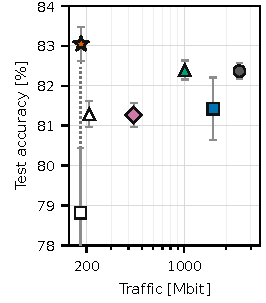
\includegraphics[width=0.245\textwidth]{figures/communication_frontier_fmnist_mlp.pdf}}\hfill
 \subfloat[Fashion-MNIST CNN]{%
  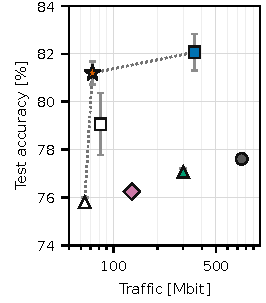
\includegraphics[width=0.245\textwidth]{figures/communication_frontier_fmnist_cnn.pdf}}\hfill
 \subfloat[CIFAR-10 CNN]{%
  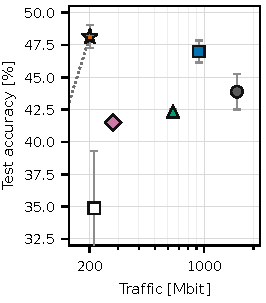
\includegraphics[width=0.245\textwidth]{figures/communication_frontier_cifar_cnn.pdf}}\hfill
 \subfloat[\rev{CIFAR-10 ResNet-14}]{%
  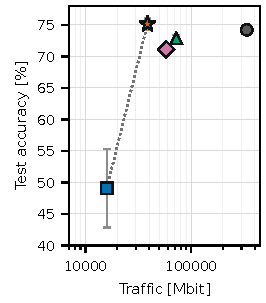
\includegraphics[width=0.245\textwidth]{figures/communication_frontier_cifar_resnet14.pdf}}
 \par\vspace{0.5mm}
 \caption{\spacerev{Ten-seed held-out communication--accuracy comparison.
 Filled markers are quality-selected and hollow markers are traffic-matched.
 Dotted lines connect points that are nondominated in the observed mean plane. Error bars show mean
 $\pm$ sample standard deviation over matched seeds.}}
 \label{fig:communication-frontier}
\end{figure*}

\begin{figure*}[t]
 \centering
 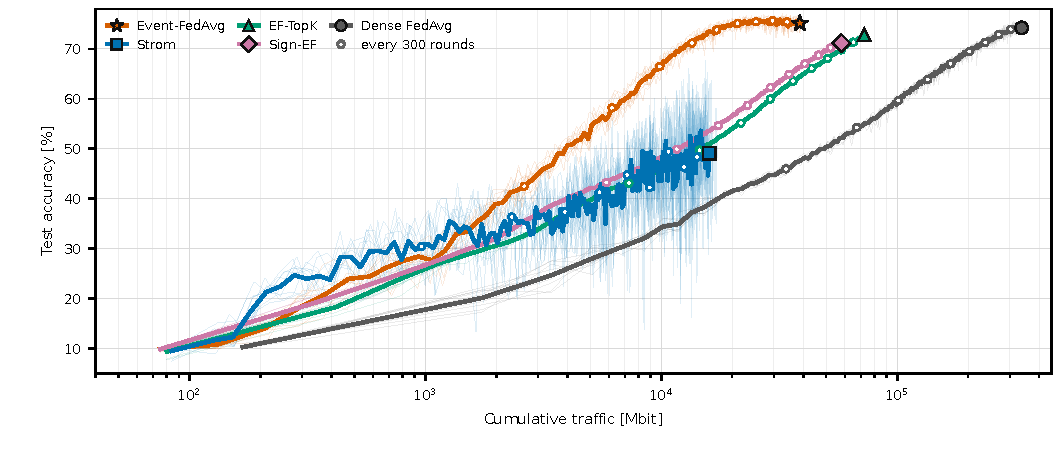
\includegraphics[width=0.90\textwidth]{figures/resnet14_communication_trajectory.pdf}
 \caption{\spacerev{CIFAR-10 ResNet-14 communication--accuracy trajectories.
 Thin curves show ten seeds, thick curves their matched-round means, open
 circles 300-round intervals, and method markers round 3,000. Traffic counts
 uploads and downlinks separately.}}
 \label{fig:resnet-communication-trajectory}
\end{figure*}

% Generated by paper/ijcnn2027/build_visuals.py. Do not edit by hand.
\begin{table*}[t]
\centering
\caption{\spacerev{Primary frozen configurations. Values are mean $\pm$ sample standard deviation over ten matched seeds. Bold marks the best mean per benchmark and metric. Lower traffic is better.}}
\label{tab:main-results}
\scriptsize
\setlength{\tabcolsep}{3pt}
\begin{tabular*}{0.99\textwidth}{@{\extracolsep{\fill}}lllrrr@{}}
\toprule
Benchmark & Selection rule & Method & Accuracy [\%] & Worst [\%] & Total [Mbit] \\
\midrule
Fashion-MNIST MLP & Event operating point & Event-FedAvg & \textbf{83.05$\boldsymbol{\pm}$0.42} & \textbf{55.0$\boldsymbol{\pm}$5.9} & 182.8$\pm$2.4 \\
 & Dense reference & Dense FedAvg & 82.37$\pm$0.20 & 51.5$\pm$2.2 & 2487.0$\pm$0.0 \\
 & \newrev{Quality-selected setting} & EF-TopK & 82.40$\pm$0.24 & 52.9$\pm$3.1 & 1010.5$\pm$0.0 \\
 & \newrev{Traffic-matched setting} & Strom & 78.82$\pm$1.62 & 40.3$\pm$12.0 & \textbf{181.5$\boldsymbol{\pm}$4.3} \\
\midrule
Fashion-MNIST CNN & Event operating point & Event-FedAvg & 81.20$\pm$0.49 & \textbf{42.5$\boldsymbol{\pm}$7.4} & \textbf{72.1$\boldsymbol{\pm}$1.0} \\
 & Dense reference & Dense FedAvg & 77.61$\pm$0.15 & 26.6$\pm$4.5 & 749.1$\pm$0.0 \\
 & \newrev{Quality-selected setting} & Strom & \textbf{82.07$\boldsymbol{\pm}$0.77} & 38.8$\pm$11.4 & 357.1$\pm$5.5 \\
 & \newrev{Traffic-matched setting} & Strom & 79.06$\pm$1.30 & 23.8$\pm$10.9 & 81.9$\pm$1.5 \\
\midrule
CIFAR-10 CNN & Event operating point & Event-FedAvg & \textbf{48.13$\boldsymbol{\pm}$0.89} & \textbf{26.0$\boldsymbol{\pm}$4.0} & \textbf{201.0$\boldsymbol{\pm}$4.0} \\
 & Dense reference & Dense FedAvg & 43.88$\pm$1.38 & 20.8$\pm$4.2 & 1586.6$\pm$0.0 \\
 & \newrev{Quality-selected setting} & Strom & 46.98$\pm$0.84 & 20.8$\pm$6.3 & 927.5$\pm$6.6 \\
 & Class-wise reference & EF-TopK & 42.32$\pm$0.22 & 24.9$\pm$1.9 & 645.2$\pm$0.0 \\
 & \newrev{Traffic-matched setting} & Strom & 34.87$\pm$4.41 & 9.8$\pm$6.0 & 214.0$\pm$17.4 \\
\midrule
CIFAR-10 ResNet-14 & Event operating point & Event-FedAvg & \textbf{75.14$\boldsymbol{\pm}$0.90} & \textbf{56.1$\boldsymbol{\pm}$3.6} & 38656.4$\pm$361.5 \\
 & Dense reference & Dense FedAvg & 74.21$\pm$0.74 & 51.7$\pm$5.5 & 336556.2$\pm$0.0 \\
 & \newrev{Quality-selected setting} & EF-TopK & 72.84$\pm$0.53 & 51.0$\pm$3.3 & 72364.7$\pm$0.0 \\
 & \newrev{Quality-selected setting} & Sign-EF & 71.16$\pm$0.26 & 48.4$\pm$3.7 & 57923.9$\pm$0.0 \\
 & \newrev{Quality-selected setting} & Strom & 49.09$\pm$6.22 & 9.2$\pm$9.7 & \textbf{15953.9$\boldsymbol{\pm}$793.1} \\
\bottomrule
\end{tabular*}
\vspace{2pt}
\parbox{0.99\textwidth}{\footnotesize \emph{Baseline sources:} dense FedAvg~\cite{mcmahan2017fedavg}, Sign-EF based on sign quantization and error feedback~\cite{seide2014onebit,bernstein2018signsgd}, EF-TopK with memory~\cite{stich2018memory,richtarik2021ef21}, and Strom threshold pulses~\cite{strom2015distributed}. \emph{Class-wise qualification:} on CIFAR-10, Event-FedAvg reaches 26.0$\pm$4.0\% mean worst-class accuracy, versus 24.9$\pm$1.9\% for the frozen EF-TopK quality point.}
\end{table*}


\section{Experimental Protocol}
\label{sec:experiments}

\textbf{Tasks and models.}
\spacerev{We evaluate ten-client image classification under strong label skew.
Fashion-MNIST uses a 25,818-parameter MLP for 150 rounds and a
14,538-parameter CNN for 80 rounds. Each client has 6,000 examples, with 55\%
from one dominant class and 5\% from each other class. CIFAR-10 uses a
20,570-parameter CNN for 120 rounds and a 175,258-parameter group-normalized
ResNet-14 for 3,000 rounds. Each client has 5,000 examples under the same class
proportions. All runs use full participation, five local SGD steps, batch size
32, and learning rate $0.1$ for Fashion-MNIST or $0.05$ for CIFAR-10. We set
$r_0=100$. Within a benchmark, every method uses the same final-round horizon.
The horizons differ across benchmarks because they were selected for the
corresponding architecture and dataset. The frozen Event-FedAvg tuples
$(\rho,\vartheta,q_0,\alpha)$ are $(0.999,0.025,0.005,0.1)$,
$(0.999,0.025,0.010,0.3)$, $(0.999,0.025,0.005,0.2)$, and
$(0.999,0.0125,0.005,0.3)$ in the listed model order.}

\textbf{Practical parameter selection.}
\spacerev{For constant retention, $\rho$ gives an approximate memory horizon
$1/(1-\rho)$. The threshold $\vartheta$ controls firing and traffic, $q_0$
controls pulse displacement, and $\alpha$ controls its decay. We jointly select
$(\vartheta,q_0)$ by final development loss and freeze all settings before
evaluation. We use $\rho=0.999$ for long memory. An ablation finds no measurable
difference from $\rho=1$ at the selected finite horizon. The complete candidate
grids, development scores, and frozen selections are included in the
reproducibility artifact.}

\spacerev{Each comparison method has a development-selected quality setting and,
when available, a traffic-matched setting. EF-TopK retains fractions $0.05$
and $0.01$. Strom's quality/traffic thresholds are $0.00125/0.02$,
$0.005/0.02$, and $0.0025/0.01$ for the three smaller models. The CIFAR-10
EF-TopK class-wise reference uses $0.05$. The compact CIFAR-10 CNN uses dense
server gain $\gamma=2$, while the ResNet-14 dense audit selects $\gamma=1.5$.
Table~\ref{tab:main-results} summarizes the primary final-round endpoints.}

\textbf{Selection and evaluation.}
We compare Event-FedAvg with dense FedAvg~\cite{mcmahan2017fedavg}, Sign-EF
based on sign quantization and error feedback
\cite{seide2014onebit,bernstein2018signsgd}, EF-TopK with memory
\cite{stich2018memory,richtarik2021ef21}, and Strom's residual-conserving
threshold pulses~\cite{strom2015distributed}. \emph{Matched local learning}
means identical client data, initialization, local steps, learning rate, and
minibatch order for every method sharing a seed. Only communication and its
server update differ.

\spacerev{Hyperparameters are selected on one development partition per
benchmark by final training loss. For dense FedAvg, server gain $\gamma$ scales
the aggregate as
$\vect{w}^{r+1}=\vect{w}^r+\gamma\sum_i p_i\vect{\delta}_i^r$. For the compact
CIFAR-10 CNN, $\gamma=2$ is selected from
$\{0.25,0.5,0.75,1,1.5,2,4\}$. The ResNet-14 choice $\gamma=1.5$ follows a
separate 900-round development audit and is frozen for the 3,000-round evaluation. For Strom and
EF-TopK, we also freeze the setting nearest Event-FedAvg in log traffic.
Table~\ref{tab:main-results} reports Event-FedAvg, dense FedAvg, and the
highest-accuracy sparse baseline selected exclusively by development loss for
each benchmark. Held-out accuracy is never used to choose this table entry.
Figure~\ref{fig:communication-frontier} contains all remaining frozen points,
including traffic-matched settings and secondary method families. Values
are means and sample standard deviations over ten paired strong-skew partitions
and training seeds. We record test cross-entropy, accuracy, worst-class
accuracy, coordinate events, and communication.}

\textbf{Communication metric.}
\spacerev{Conservative bidirectional traffic counts uploads and an individual
downlink to every client. It includes headers, addresses, signs or values,
initial synchronization, per-round requests, and the smaller of ordered replay
and a checkpoint. Dense values use 32 bits. The same rule applies to every
method.}

\textbf{Alignment study.}
\spacerev{A Fashion-MNIST MLP $2\times2$ study crosses IID or strong non-IID
data with one or five local steps while holding other settings fixed. For ten
paired seeds, rounds $1,5,10,\ldots,150$ are audited by independently rerunning
the same trajectory. Exact full-client gradients are evaluated after the event
decision, so diagnostics cannot alter later crossings.}

\textbf{Mechanism audits.}
\actionrev{The complete Event-FedAvg operator combines cross-round encoder
memory, leakage, full reset, and separate trigger and model-update scales.
Baseline comparisons cannot identify which internal choice matters. We
therefore audit four changes at the compact CIFAR-10 CNN operating point:
memoryless state, no leakage ($\rho=1$), subtractive reset that retains
overshoot, and coupling $q_r$ to the threshold. For the memoryless and
subtractive families, one threshold is selected on the development partition
by minimum log-distance to the frozen operator's total traffic. The selected
thresholds are $0.010$ and $0.025$, respectively. Neither is at a search-grid
boundary. They are then frozen for the same ten paired held-out seeds. All
other training, quantum, and communication settings remain unchanged.}

\section{Results and Discussion}
\label{sec:results}

\spacerev{Figure~\ref{fig:communication-frontier} compares total bidirectional
traffic and accuracy over the same ten matched seeds per panel. Filled markers
show quality-selected settings and hollow markers show traffic-matched settings.
Table~\ref{tab:main-results} reports the three primary final-round endpoints
per benchmark, while the figure retains all evaluated operating points.}

% Generated by paper/ijcnn2027/build_alignment_factorial.py; do not edit.
\begin{table*}[t]
\centering
\caption{\actionrev{Fashion-MNIST MLP alignment audit. Values are mean $\pm$ sample standard deviation over ten paired seeds and 31 independently audited checkpoints per seed.}}
\label{tab:alignment-factorial}
\scriptsize
\setlength{\tabcolsep}{3pt}
\begin{tabular*}{0.99\textwidth}{@{\extracolsep{\fill}}lrrrrrrr@{}}
\toprule
Setting & $\widehat{\kappa}_{\mathcal A}$ & $\Delta F_r<0$ [\%] & $\widehat\beta_r=0$ [\%] & $\widehat{\mathcal D}_{\mathcal A}$ & $\widehat{\mathcal V}_{\mathcal A}$ & $\overline B_{\mathcal A}$ & $\overline L_{\mathcal A}$ \\
\midrule
IID, $E=1$ & 10.36$\pm$0.23 & 96.1$\pm$1.4 & 87.7$\pm$2.0 & 0.063$\pm$0.002 & 20.0$\pm$0.6 & -0.25$\pm$0.04 & -22.1$\pm$1.1 \\
IID, $E=5$ & 45.31$\pm$1.66 & 94.8$\pm$4.1 & 91.9$\pm$3.8 & 0.021$\pm$0.001 & 83.7$\pm$1.9 & -5.65$\pm$0.46 & -59.2$\pm$3.4 \\
Strong non-IID, $E=1$ & 20.14$\pm$0.87 & 87.4$\pm$4.4 & 92.3$\pm$1.7 & 0.029$\pm$0.004 & 158.1$\pm$4.3 & -350.31$\pm$18.17 & -90.2$\pm$8.5 \\
Strong non-IID, $E=5$ & 35.40$\pm$1.52 & 69.7$\pm$9.3 & 93.5$\pm$3.4 & 0.022$\pm$0.003 & 306.6$\pm$4.6 & -678.29$\pm$44.63 & 400.5$\pm$24.3 \\
\bottomrule
\end{tabular*}
\vspace{2pt}
\parbox{0.99\textwidth}{\scriptsize $\widehat\beta_r=[8\lVert\vect{g}^r\rVert_2^2-A_r]_+$. $\widehat{\mathcal D}_{\mathcal A}$ and $\widehat{\mathcal V}_{\mathcal A}$ are the sampled alignment-defect and event-curvature terms in~\eqref{eq:empirical-theorem-diagnostics}. $\overline B_{\mathcal A}$ and $\overline L_{\mathcal A}$ are the normalized $q_r$-weighted heterogeneity and local-mismatch terms.}
\end{table*}


\newrev{Table~\ref{tab:main-results} summarizes the ten-seed tradeoffs. Across
the three smaller models, Event-FedAvg is either the most accurate method or
within $0.87$ percentage points of it while using substantially less traffic
than the development-selected comparison. The clearest smaller-model result is
on the CIFAR-10 CNN, where Event-FedAvg improves on dense FedAvg by $4.25$
points while using $12.7\%$ of its traffic. Figure~\ref{fig:communication-frontier}
provides the broader comparison without duplicating those points in the table.}

\actionrev{The Event-FedAvg-to-dense traffic ratios remain favorable under a
logical-broadcast accounting model. From Fashion-MNIST MLP through ResNet-14,
they are $2.4\%$, $3.1\%$, $4.1\%$, and $3.8\%$, compared with $7.4\%$,
$9.6\%$, $12.7\%$, and $11.5\%$ under conservative unicast. This sensitivity
uses the already recorded packet streams and requires no retraining. It does
not establish the ranking under every network or multicast implementation.}

\spacerev{On ResNet-14, Event-FedAvg reaches $75.14\pm0.90\%$ accuracy and
$56.1\pm3.6\%$ worst-class accuracy at $38.66\pm0.36$ Gbit. Dense FedAvg
reaches $74.21\pm0.74\%$ and $51.7\pm5.5\%$ at $336.56$ Gbit. The paired
accuracy advantage is $0.93$ points with a 95\% interval of $[0.17,1.69]$ points
and holds for seven of ten pairs. Thus Event-FedAvg uses $11.5\%$ of dense traffic.}

\actionrev{This is an operating-point comparison, not evidence that sparsity
alone causes the accuracy gain. Event-FedAvg changes both the transmitted
representation and the induced server update, including a decaying quantum,
whereas the dense reference uses the development-selected constant gain from
the preceding audit.}

\spacerev{Figure~\ref{fig:resnet-communication-trajectory} shows that
Event-FedAvg reaches its accuracy plateau by about round 1,800, while dense
FedAvg, EF-TopK, and Sign-EF continue to improve. Event-FedAvg reaches
intermediate accuracy levels with less traffic than EF-TopK and dense FedAvg.
Strom fluctuates more across all seeds, plausibly because its fixed residual
pulse couples threshold and update magnitude in this synchronous adaptation.
This does not imply general instability of the original asynchronous method.
For the other methods, shrinking 300-round gains indicate slowing progress.
The fixed 3,000-round endpoint therefore gives the baselines more time to close
the earlier gap, but it remains a finite-horizon comparison rather than a
convergence claim.}

\textbf{Mechanism audit.}
\actionrev{The four controlled changes separate memory, leakage, reset, and
scale separation at the selected compact CIFAR-10 operating point.} Removing leakage
($\rho=1$) \rev{produces nearly the same result as} the frozen setting at this resolution
($48.32\pm1.05\%$ versus $48.25\pm1.07\%$). Coupling the quantum and trigger
at $0.025$ instead reduces accuracy to $18.42\pm7.33\%$. This supports their
independence for the selected operating point, not a universal claim that every
coupled schedule fails.

\begin{table}[t]
\centering
\caption{\actionrev{Compact CIFAR-10 CNN operator audit over ten paired held-out seeds. Values are mean $\pm$ sample standard deviation.}}
\label{tab:operator-ablation}
\scriptsize
\setlength{\tabcolsep}{3.5pt}
\begin{tabular}{@{}lrrr@{}}
\toprule
Encoder & Accuracy [\%] & Worst [\%] & Total [Mbit] \\
\midrule
Persistent, full reset & 48.13$\pm$0.89 & \textbf{26.0$\pm$4.0} & 201.0$\pm$4.0 \\
Memoryless, full reset & 36.49$\pm$1.45 & 7.4$\pm$3.4 & \textbf{194.2$\pm$5.4} \\
Persistent, subtractive & \textbf{48.55$\pm$0.82} & 25.2$\pm$5.3 & 209.2$\pm$4.5 \\
\bottomrule
\end{tabular}
\end{table}


\actionrev{Table~\ref{tab:operator-ablation} completes the audit by asking whether the temporal state or
reset rule explains the selected operating point. Removing cross-round memory
reduces paired accuracy by $11.64$ points, with a 95\% confidence interval of
$[-12.79,-10.49]$ points and a loss on every seed, although traffic is $3.3\%$
lower. Persistent accumulation therefore contributes information beyond event
rate control in this audit. Subtractive reset changes accuracy by only $+0.42$
points, with a 95\% confidence interval of $[-0.01,0.85]$ points, while using
$4.1\%$ more traffic. Thus the experiment identifies persistence as the
important mechanism at this operating point. It does not establish predictive
superiority of full reset. We retain full reset because it defines the tested
operator and yields the bounded-state invariant and disjoint blocks used in
the analysis.}

\spacerev{Table~\ref{tab:alignment-factorial} supports two main observations.
First, aggregate events usually retain positive first-order alignment. Second,
stronger heterogeneity and more local steps enlarge the gap between alignment
and realized objective descent. The remaining columns diagnose why this gap
appears. The table reports ten seeds and 31 audited
checkpoints per seed at rounds $1,5,10,\ldots,150$. Each audit independently
reruns training from the same initialization. Its
$\widehat\kappa_{\mathcal A}$ is the trajectory ratio in
\eqref{eq:empirical-alignment-ratio}, not mean $A_r$ or theoretical $\kappa$.
\actionrev{The diagnostic columns separate first-order alignment, realized
descent, the sampled theorem terms, and the two signed decomposition
components most directly affected by local depth and heterogeneity. Across the
four cells, $96.1$--$99.0\%$ of audited aggregates have positive first-order
alignment.}}

\spacerev{$\overline B_{\mathcal A}$ exposes adverse heterogeneity, while
$\overline L_{\mathcal A}$ shows that increasing local steps from one to five
acts differently under IID and non-IID data. Under strong non-IID data, five
steps retain frequent positive alignment but produce fewer objective decreases
and a larger remainder. No pulse opposes its local-update proxy in the
$1{,}240$ snapshots, so the recorded memory-opposition term is zero. This is a
finite-trajectory observation, not a general encoder property or proof of
Assumption~\eqref{eq:alignment-assumption-paper}.}

\spacerev{For the fixed reference $\kappa_0=8$, most checkpoints have zero
realized defect. Nonzero $\widehat{\mathcal D}_{\mathcal A}$ values show that a
positive trajectory average does not exclude unfavorable rounds.
$\widehat{\mathcal V}_{\mathcal A}$ increases with non-IID data and five local
steps, matching the larger gap between first-order alignment and objective
descent. These sampled diagnostics support the proposed finite-horizon
mechanism but do not estimate the required conditional expectation or unknown
global smoothness constant.}

\section{Limitations}
\label{sec:limitations}

\spacerev{The evaluation covers synchronous full participation, ten clients,
two image datasets, and development-selected configurations. Ten paired seeds
measure matched-run variation but do not provide simultaneous inference over
all comparisons. Selection on one development partition does not quantify
hyperparameter-selection uncertainty across alternative development samples.
The alignment study varies only partitioning and local steps
around one Fashion-MNIST setting. The theorem assumes rather than proves
aggregate alignment and makes no asymptotic claim. Broader data, participation,
and hyperparameter regimes remain open. Finally, software bit counts do not
measure latency, packet loss, asynchronous behavior, or hardware energy.}

\section{Conclusion}
\label{sec:conclusion}

\spacerev{Event-FedAvg converts accumulated local-model changes into sparse
signed events while preserving exact synchronization. We bound its state and
event count and identify aggregate alignment as the condition connecting events
to finite-horizon progress. Among the evaluated frozen configurations, it is
nondominated in the observed mean communication--accuracy plane across four
ten-client image-classification settings. The mechanism audit identifies
persistent accumulation and independent update resolution as influential at
the selected compact-CNN operating point. It does not show predictive
superiority of full over subtractive reset. On CIFAR-10 ResNet-14, it improves mean accuracy over
development-tuned dense FedAvg by $0.93$ points with $8.7\times$ less traffic.
The alignment study shows why positive first-order alignment need not imply an
objective decrease under stronger heterogeneity and more local steps. Future
work should test partial participation, asynchronous operation, and measured
system-level communication and energy.}

\begin{samepage}
\section*{Acknowledgment}
\actionrev{OpenAI ChatGPT and Codex~\cite{openai2026chatgpt} assisted language
editing throughout and development of experimental and validation code. The
authors designed the study, and the authors verified all scientific claims and
take responsibility for the content. AI output did not serve as scientific
evidence.}
\end{samepage}

\begingroup
% IEEEtran selects \footnotesize inside the bibliography environment.  Keep
% the references compact enough for the conference page limit.
\let\footnotesize\scriptsize
\bibliographystyle{IEEEtran}
\bibliography{references}
\endgroup

\end{document}
